\chapter{Introduction}

\section{Image}

An image is a two-dimensional function that represents a measure of some characteristics such as brightness or color of a viewed scene. An image is projection of a 3D scene into a 2D projection plane. It can be defined as a two-variable function $f(x,y)$ where for each position $(x,y)$ in the projection plane, $f(x,y)$ defines the light intensity at this point.

\subsection{Analog Image}

An Analog Image can be mathematically represented as a continuous range of values representing positions and intensity. An Analog Image is characterised by a physical magnitude varying continuously in space.

E.g.: The image produced on the screen of a CRT monitor is analog in nature.

\subsection{Digital Image}

A Digital Image is composed of picture elements called \textit{pixels}. Pixels are the smallest sample of an image. A pixel represents the brightness at one point. Conversion of an analog image into a digital image involves two important operations, namely, sampling and quantisation, which are illustrated in Fig: \ref{Digital-to-analog}.

\begin{figure}[h]
    \centering
\tikzset{every picture/.style={line width=0.75pt}} %set default line width to 0.75pt        

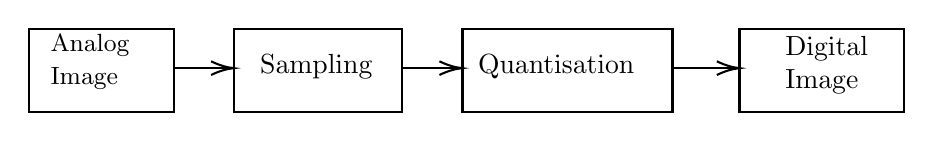
\begin{tikzpicture}[x=0.75pt,y=0.75pt,yscale=-1,xscale=1]
%uncomment if require: \path (0,300); %set diagram left start at 0, and has height of 300

%Shape: Rectangle [id:dp5271710061639749] 
\draw   (60,95) -- (129.8,95) -- (129.8,135) -- (60,135) -- cycle ;
%Shape: Rectangle [id:dp38336255974485245] 
\draw   (158.8,95) -- (239.8,95) -- (239.8,135) -- (158.8,135) -- cycle ;
%Shape: Rectangle [id:dp6224918178723147] 
\draw   (269,95) -- (370.16,95) -- (370.16,135) -- (269,135) -- cycle ;
%Shape: Rectangle [id:dp8433034035458677] 
\draw   (402.47,95) -- (481.8,95) -- (481.8,135) -- (402.47,135) -- cycle ;
%Straight Lines [id:da09940164773903648] 
\draw    (129.8,114) -- (156.8,114) ;
\draw [shift={(158.8,114)}, rotate = 180] [color={rgb, 255:red, 0; green, 0; blue, 0 }  ][line width=0.75]    (10.93,-3.29) .. controls (6.95,-1.4) and (3.31,-0.3) .. (0,0) .. controls (3.31,0.3) and (6.95,1.4) .. (10.93,3.29)   ;
%Straight Lines [id:da6636252308653761] 
\draw    (239.8,114) -- (266.8,114) ;
\draw [shift={(268.8,114)}, rotate = 180] [color={rgb, 255:red, 0; green, 0; blue, 0 }  ][line width=0.75]    (10.93,-3.29) .. controls (6.95,-1.4) and (3.31,-0.3) .. (0,0) .. controls (3.31,0.3) and (6.95,1.4) .. (10.93,3.29)   ;
%Straight Lines [id:da7001004518882727] 
\draw    (370.16,114) -- (400.47,114) ;
\draw [shift={(402.47,114)}, rotate = 180] [color={rgb, 255:red, 0; green, 0; blue, 0 }  ][line width=0.75]    (10.93,-3.29) .. controls (6.95,-1.4) and (3.31,-0.3) .. (0,0) .. controls (3.31,0.3) and (6.95,1.4) .. (10.93,3.29)   ;

% Text Node
\draw (69,96) node [anchor=north west][inner sep=0.75pt]   [align=left] {{\small Analog}\\{\small Image}};
% Text Node
\draw (170,106) node [anchor=north west][inner sep=0.75pt]   [align=left] {Sampling};
% Text Node
\draw (275,106) node [anchor=north west][inner sep=0.75pt]   [align=left] {Quantisation};
% Text Node
\draw (423.03,97) node [anchor=north west][inner sep=0.75pt]   [align=left] {Digital\\Image};

\end{tikzpicture}
\caption{Digital Image from Analog Image}
    \label{Digital-to-analog}
\end{figure}

\subsubsection{Advantages of Digital Images:}
The advantages of Digital Images are summarised below:
\begin{itemize}
    \item The Processing of images is faster and cost-effective.
    \item Digital Images can be effectively stored and efficiently transmitted from one place to another.
    \item When shooting a digital image, one can immediately see if the image is good or not.
    \item Copying a digital image is easy. The quality of digital image will not be degraded even if it is copied for several times.
    \item Whenever the image is in digital format, the reproduction of the image is both faster and cheaper.
    \item Digital technology offers plenty of scope for versatile image manipulation.
\end{itemize}

\subsubsection{Drawbacks of Digital Images:}
Some of the drawbacks of Digital Images are summarised below:
\begin{itemize}
    \item Misuse of copyright has become easier because images can be copied from Internet just by clicking the mouse a couple of times.
    \item A digital file cannot be enlarged beyond a certain size without compromising on quality.
    \item The memory required to store and process good-quality digital images is very high.
    \item For real-time implementation of digital-image-processing algorithms, the processor has to be very fast because the volume of data is very high.
\end{itemize}

\section{Digital Image Processing}

The processing of an image by means of a computer is generally termed as \textbf{Digital Image Processing}.

The Advantages of computers for the processing of images are summarised below:
\begin{itemize}
    \item \textbf{Flexibility and Adaptability:} The main advantage of digital computers when compared to analog electronic and optical information processing devices is that no hardware modifications are necessary in order to reprogram digital computers to solve different tasks. This feature makes digital computers an ideal devices for processing image signals adaptively.
    \item \textbf{Data Storage and Transmission:} With the development of different image-compression algorithms, the digital data can be effectively stored. The digital data within computers can be easily transmitted from one place to another.
\end{itemize}

The only limitation of Digital Image and Digital Image Processing are memory and processing speed capabilities of computers. Different Image-Processing techniques include \textit{Image Enhancements, image restoration, image fusion} and \textit{image watermarking}.

\section{Digital Image Representation}

A digital image is a two-dimensional discrete signal.
A digital image is also an $NxN$ array of elements.
Each element in the array is a number which represents the sampled intensity.
For e.g. : The representation of a $4x4$ image in matrix format is shown in Fig: \ref{matrix_view}.

\begin{figure}[h]
    
\begin{equation*}
    \begin{bmatrix}
    1 & 1 & 1 & 1\\
    1 & 1 & 1 & 1\\
    0 & 0 & 0 & 0\\
    0 & 0 & 0 & 0
    \end{bmatrix}
\end{equation*}

    \caption{Digital Image Representation}
    \label{matrix_view}
\end{figure}

Converting an image into a digital format can be done either with a digital camera, or by a scanner.
Digital images can be created directly on a computer screen.
However, it is restricted both in spatial coordinates (sampling) and in its allowed intensities (quantisation).

\subsection{Neighbours of a Pixel}
A pixel will have four neighbours if the neighbours exist in the EAST, WEST, NORTH and SOUTH directions. The four neighbours of the pixel `P' are represented in Fig: \ref{neighboursOfPixel}.

\begin{figure}[h]
    \centering

    \tikzset{every picture/.style={line width=0.75pt}} %set default line width to 0.75pt        

    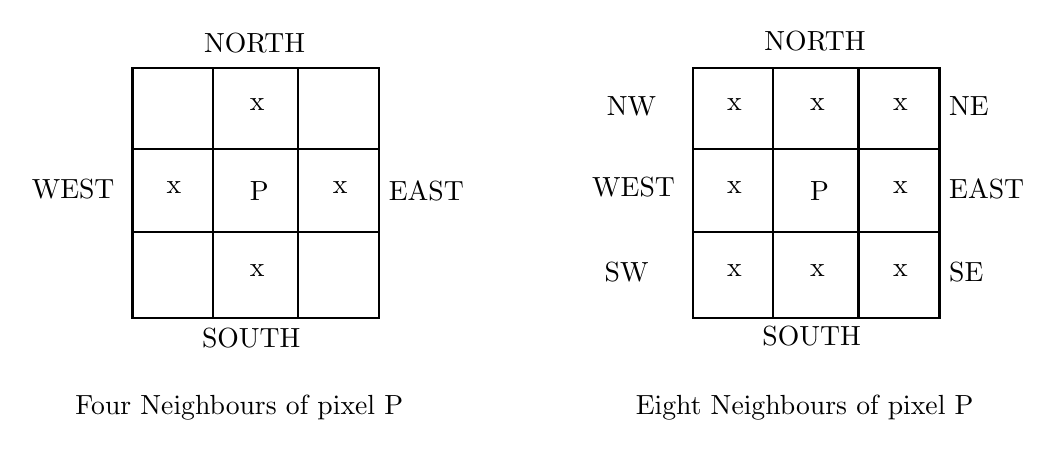
\begin{tikzpicture}[x=0.75pt,y=0.75pt,yscale=-1,xscale=1]
    %uncomment if require: \path (0,300); %set diagram left start at 0, and has height of 300
    
    %Shape: Rectangle [id:dp6330616545415024] 
    \draw   (51,51) -- (169.8,51) -- (169.8,171.2) -- (51,171.2) -- cycle ;
    %Shape: Rectangle [id:dp5493809441405086] 
    \draw   (51,90) -- (169.8,90) -- (169.8,130) -- (51,130) -- cycle ;
    %Shape: Rectangle [id:dp4349468061351809] 
    \draw   (89.8,51) -- (130.8,51) -- (130.8,171.2) -- (89.8,171.2) -- cycle ;
    
    %Shape: Rectangle [id:dp08063473849200564] 
    \draw   (321,51) -- (439.8,51) -- (439.8,171.2) -- (321,171.2) -- cycle ;
    %Shape: Rectangle [id:dp7254088029401085] 
    \draw   (321,90) -- (439.8,90) -- (439.8,130) -- (321,130) -- cycle ;
    %Shape: Rectangle [id:dp4119143208436029] 
    \draw   (359.8,51) -- (400.8,51) -- (400.8,171.2) -- (359.8,171.2) -- cycle ;
    
    
    % Text Node
    \draw (106,104) node [anchor=north west][inner sep=0.75pt]   [align=left] {P};
    % Text Node
    \draw (146,104) node [anchor=north west][inner sep=0.75pt]   [align=left] {x};
    % Text Node
    \draw (66,104) node [anchor=north west][inner sep=0.75pt]   [align=left] {x};
    % Text Node
    \draw (106,144) node [anchor=north west][inner sep=0.75pt]   [align=left] {x};
    % Text Node
    \draw (106,64) node [anchor=north west][inner sep=0.75pt]   [align=left] {x};
    % Text Node
    \draw (376,104) node [anchor=north west][inner sep=0.75pt]   [align=left] {P};
    % Text Node
    \draw (416,104) node [anchor=north west][inner sep=0.75pt]   [align=left] {x};
    % Text Node
    \draw (336,104) node [anchor=north west][inner sep=0.75pt]   [align=left] {x};
    % Text Node
    \draw (376,144) node [anchor=north west][inner sep=0.75pt]   [align=left] {x};
    % Text Node
    \draw (376,64) node [anchor=north west][inner sep=0.75pt]   [align=left] {x};
    % Text Node
    \draw (336,144) node [anchor=north west][inner sep=0.75pt]   [align=left] {x};
    % Text Node
    \draw (336,64) node [anchor=north west][inner sep=0.75pt]   [align=left] {x};
    % Text Node
    \draw (416,64) node [anchor=north west][inner sep=0.75pt]   [align=left] {x};
    % Text Node
    \draw (416,144) node [anchor=north west][inner sep=0.75pt]   [align=left] {x};
    % Text Node
    \draw (22,207) node [anchor=north west][inner sep=0.75pt]   [align=left] {Four Neighbours of pixel P};
    % Text Node
    \draw (292,207) node [anchor=north west][inner sep=0.75pt]   [align=left] {Eight Neighbours of pixel P};
    % Text Node
    \draw (1,103) node [anchor=north west][inner sep=0.75pt]   [align=left] {WEST};
    % Text Node
    \draw (83,175) node [anchor=north west][inner sep=0.75pt]   [align=left] {SOUTH};
    % Text Node
    \draw (173,104) node [anchor=north west][inner sep=0.75pt]   [align=left] {EAST};
    % Text Node
    \draw (84,33) node [anchor=north west][inner sep=0.75pt]   [align=left] {NORTH};
    % Text Node
    \draw (271,102) node [anchor=north west][inner sep=0.75pt]   [align=left] {WEST};
    % Text Node
    \draw (353,174) node [anchor=north west][inner sep=0.75pt]   [align=left] {SOUTH};
    % Text Node
    \draw (443,103) node [anchor=north west][inner sep=0.75pt]   [align=left] {EAST};
    % Text Node
    \draw (354,32) node [anchor=north west][inner sep=0.75pt]   [align=left] {NORTH};
    % Text Node
    \draw (443,143) node [anchor=north west][inner sep=0.75pt]   [align=left] {SE};
    % Text Node
    \draw (443,63) node [anchor=north west][inner sep=0.75pt]   [align=left] {NE};
    % Text Node
    \draw (278,63) node [anchor=north west][inner sep=0.75pt]   [align=left] {NW};
    % Text Node
    \draw (277,143) node [anchor=north west][inner sep=0.75pt]   [align=left] {SW};
    
    
    \end{tikzpicture}
    \caption{Neighbours of Pixels}
    \label{neighboursOfPixel}
\end{figure}

\section{Classification of Digital Images}

Digital Images can be broadly classified into two types and they are:
\begin{enumerate}
    \item Raster Image
    \item Vector Image
\end{enumerate}

\subsection{Raster Image or Bitmap Image}

\begin{itemize}
    \item A raster image file is generally defined as a rectangular array of regularly sampled values known as pixels.
    \item Scanned graphics and web graphics are the most common forms of raster images.
    \item Raster images are mapped to grids which are not easily scalable.
    \item A raster image is resolution dependent because it contains a fixed number of pixels that are used to create the image. Since there are a fixed and limited number of pixels, raster image will lose its quality if it is enlarged beyond that number of pixels as the computer will have to `make up' for the missing information.
    \item When an image is zoomed by a factory of 24 (say), the clarity is lost.
    \item Bitmaps are used for photorealistic images, and therefore, involve complex color variations.
    \item Raster images can show well the gradations of color and detailed images such as photographs.
    \item The spatial resolution of a raster image is determined by the resolution of the acquisition device and the quality of the original data source.
\end{itemize}

Common Raster Image formats include:
BMP (Windows Bitmap), PCX (Paintbrush), TIFF (Tag Interleave Format), JPEG/JPG (Join Photographics Expert Group), GIF (Graphics Interchange Format), PNG (Portable Network Graphics), PSD (Adobe Photoshop) and CPT (Corel PhotoPaint)

\subsection{Vector Image}

\begin{itemize}
    \item A vector image is defined by objects which are made of lines and curves that are mathematically defined in the computer.
    \item A vector can have various attributes such as line thickness, length and color.
    \item Vector images are mathematically defined and hence, they are scalable.
    \item This implies that vectors can be printed at any size, on any output device, at any resolution, without losing the detail and without altering the resultuion of the image.
    \item A Vector image, when zoomed by a factor of 24 (say), shows no distortion and clarity is preserved.
    \item Vector images can be scaled by several factors without altering the resolution of the image.
    \item Vector images are suitable for typography, line art and illustrations.
\end{itemize}

\section{Image Types}

Images can be broadly classified under four categories:
\begin{enumerate}
    \item Black \& White or Binary Image.
    \item Grayscale Image.
    \item Color Image.
    \item Multispectral Image.
\end{enumerate}

\subsection{Binary Image}
\begin{itemize}
    \item Binary Images take only two values, i.e. either `0' or `1'.
    \item The brightness graduation cannot be differentiated in Binary Images.
    \item A Grayscale image can be converted to Binary Image by the threshold operation.
    \item Geometric Properties of an object can be easily extracted from a binary image.
\end{itemize}

\subsection{Grayscale Image}
\begin{itemize}
    \item Grayscale images contain only brightness information.
    \item Each Pixel value in a grayscale image corresponds to an amount or quantity of light.
    \item The brightness graduation can be differentiated in a grayscale image.
    \item Each pixel is represented by a `byte' or` word'.
    \item An 8-bit image will have a brightness variation from 0 to 255 where `0' represents Black and `255' represents White.
\end{itemize}

\subsection{Color Image}
\begin{itemize}
    \item A color image has three values per pixel and they measure the intensity and chrominance of light.
    \item Each pixel is a vector of color components.
    \item Common Color spaces are RGB (Red, Green, Blue), HSV (Hue, Saturation, Value) and CMYK (Cyan, Magenta, Yellow, Black).
    \item The typical uncompressed data rate of a color image is three times the data rate of an uncompressed grayscale image.
\end{itemize}

\subsection{Volume Image}
\begin{itemize}
    \item A three-dimensional image is an example ofvolume image.
    \item The volume image can be optained from some medical imaging equipment in which the individual data points are called `voxels'.
    \item Voxel stands for Volume Pixel.
    \item A CAT Scan is an example of Volume Image.
\end{itemize}

\subsection{Range Image}

\begin{itemize}
    \item Range Images are a special class of digital images.
    \item Each pixel ofa range image expresses the distance between a known reference frame and a visible point in the screen.
    \item The range image reproduces the 3D structure of a scene.
    \item Range images are also referred as depth images.
\end{itemize}

\section{Image File Formats}

\begin{itemize}

    \item A digital image is often encoded in the form of binary files for the purpose of storage and transmission.
    \item A file format is a method used to store digital data and different file formats exist for storing images.
    \item Different file formats may compress the image data by differing amounts.
    \item Whatever be the format, the image file consists of two parts:
    \begin{enumerate}
        \item File Header
        \item Image Data
    \end{enumerate}
\end{itemize}

\subsubsection{Common Image File Formats:}

Various image file formats are widely used for the purpose fo digital storage and retrieval. Each of these file formats posses certain characteristics which makes them valid for various applications.
These include: GIF, JPEG/JPG, PNG, TIFF, PSD, EPS.

\subsection{File Header}

The Header part contains some of the vital information like format or version identification, width and height of the image, type of the image (binary, grayscale, color image) and image data format which specifies the order in which pixel values are stored in the image data section.
The header also specifies the type of compression mechanism.
The length of the File Header is often fixed.
The header information must provide all the necessary information to reconstruct the original data and its origanisation from the stored data.

\section{Applications of Digital Image Processing:}
Digital Image Processing is widely used in different fields like:
\begin{enumerate}
    \item Medicine
    \item Forensics
    \item Remote Sensing
    \item Communications
    \item Automobiles.
\end{enumerate}